\documentclass[11 pt, a4paper]{article}

\usepackage{graphicx, amsmath,amssymb,amsfonts, dsfont, hyperref, framed, enumitem,color}
\usepackage[hmargin=2cm,vmargin=2cm]{geometry}
\usepackage{parskip} 
\usepackage{listings}
\usepackage{float}
\usepackage{subfig}
\linespread{1.25}
\renewcommand{\labelitemii}{$\circ$}

\begin{document}
\begin{titlepage}
\begin{center}

\begin{figure}[H]
\centering
\includegraphics[width=125mm]{Leeds_Logo.pdf}
\end{figure}

\vspace{4cm}
{\LARGE \textbf{MATH3001}: Project in Mathematics}\\

\vspace{1cm}
{\Huge \textbf{Flood Analysis}:Assessing and communicating mitigation of river floods to policy makers and the general public}\\
\vspace{5cm}
\textbf{Abbey Chapman}\\
ID: 201005685\\
\vfill
School of Mathematics\\
University of Leeds\\
2018/2019
\end{center}
\end{titlepage}

\tableofcontents 
\noindent \hrulefill

\newpage
\section{Introduction}
This project aims to use the analysis of flood data for multiple floods of a range of rivers as provided under the Freedom of Information Act by the Environment Agency and subsequently analyse the cost benefits of various proposed flood mitigation plans. \\
Major flooding causes have had a huge detremental affect on the UKs' economy, it's business and the community at large. "In England and Wales alone, over 4 million people and properties valued at over £200 billion are at risk"\cite{1} and the cost of the Boxing Day 2015 floods was estimated to have topped \pounds5 billion\cite{2}.Hence, it is our goal to provide analysis of flood data and various flood mitigation approaches to assist policy makers, businesses and the general public in reducing the negative affects of floods.\\

Specifically we will explore:\\
\begin{framed}
\begin{itemize}
\item The possible flood mitigation plans that could be used.
\item The 2015 Boxing Day floods of the Rivers Aire, Calder and Don. This analysis will be done by the entire group.
\item The cost benefits of proposed flood mitigation plans to prevent any future floods along these rivers.
\item The 2012 November floods of the River Avon in both Warwick and Stratford-upon-Avon. This analysis will be done individually.
\item The cost benefits of proposed flood mitigation plans to prevent any future floods along the River Avon and specifically in these locales.
\end{itemize}
\end{framed}
Questions to be resolved:\\
\textbf{How do I attach graphs, code, excel spreadsheets e.t.c.}\\
\textbf{Should I reference Toms' Github or the EA for Aire, Calder and Don data?}\\
\textbf{How to reference Onno's project outline, its not publicly available?}\\


\newpage
\section{Flood Mitigation}
\subsection{The Meaning of Flood Mitigation}
First of all, it should be made clear what Flood Mitigation actually is. To mitigate a flood is to reduce the amount of flooding, and thereby the damage as a result of such flooding, caused when a river breaks its banks.\\ 
This has been attempted since the very origins of non-nomadic humanity as the negative financial and social repercussions of a large flood (such as loss of property, crops, infrastructure and even life) are severe. Early examples of attempts to mitigate floods include the construction of stilt-houses by the Yue people in Ancient China around 7000 years ago.\cite{3}\\ 
In the modern world, we now have access to a vast array of possible flood mitigation schemes due to factors such as improvements in engineering and the implementation of a centralised  government with access to large sums of money with wich to implement flood mitigation schemes as well as the legal authority with which to do so.\\
In the course of this report, we will be investigating the effectiveness of such schemes at realistically reducing the volume of water discharged during a flood and thereby the cost effectiveness also, in the hopes that policy makers could make use of such analysis when implementing flood mitigation proposals.

\subsection{Possible Methods of Flood Mitigation}
Examples of possible Flood Mitigation strategies include, but are not limited to:\\
\begin{itemize}
\item High Flood Walls: increases the total volume of water a river can hold before it starts to flood.
\item River-Bed wWdening: similar to high flood walls, it increases the capacity of the river itself.
\item Flood Plain Enhancement: increases the water retention of the ground itself within places at risk of flooding.
\item Natural Flood Management. This method includes examples such as:
\begin{itemize}
\item Tree Planting:  improves the water retention of the ground as trees 'drink' water.
\item Peat Restoration: improves the water retention of the ground.
\item Flow Attenuation Features: includes examples such as 'leaky dams' (like the ones that a beaver colony would build) that slow the flow of the river.
\end{itemize}
\item Sustainable Drainage Systems. This includes: \cite{4}
\begin{itemize}
\item Green Roofs: roofs that are comprised of vegetation on top of a drainage system.
\item Rainwater Harvesting: collects rainwater from roofs and thereby prevents the rainwater from contributing to any possible flooding. One such way of harvesting rainwater is the use of water butts, which collects rainwater running off roofs.
\item Permeable Pavements: pavements that allow rainwater to pass through the hard surface (preventing it from gathering and causing any potential flooding) where it will be stored to either be released into the ground at a sustainable rate (i.e. a rate that will not cause the ground to become waterlogged and thereby cause flooding) or into a drainage system that will transport the rainwater away from the immediate vacinity.
\item Soakways: similar to permeable pavements, there aim is to store rainwater run off from a development so it can then be fed into the ground.
\item Filter Strips: used in order to transport rainwater run off to systems such as soakways or streams.
\item Trenches: similar to filter strips but with the aim of storing rainwater to gradually be released into the ground as opposed to transporting the rainwater to an alternative storage entity.
\item Swales: akin to trenches but whereas trenches are filled with material like rubble, Swales are filled with vegetation and can be used both to store and release water as well as transport it.
\item Bioretention: also known as rain gardens, are shallow bowls in the ground that capture, and more significantly, treat rainwater.
\item Geocellular/Modular Systems: situated below the ground, these, much like permeable pavements, can either infiltrate rainwater run off into the ground or store said run off until it can be transported to a drainage system.
\item Infiltration Basins: comparable to bioretention methods, infiltration basins store run off for it to then be released into the ground but do not treat the water.
\item Detention Basins: temporarily store rainwater run off and, through a controlled flow, mitigates the force of the flow.
\item Ponds: unlike infiltration basins, detention basins and bioretention methods, ponds are permanent bodies of water. Ponds mitigate floods if they are low-lying, i.e. they can accept an addition of a high volume of water before they break their banks.
\item Wetlands: marshland, these works by helping to store water before it slowly enters the ground and also by reducing water flow.
\end{itemize}
\item The drawing down of drinking water reservoirs before predicted heavy rainfall: reduces the total volume of fluid stored in reservoirs thereby allowing said reservoir to accomodate a larger volume of rain fall before it fills up and begins to flood.
\end{itemize}

\newpage
\section{Analysis of the 2015 Boxing Day floods}
Here, we will be analysing flood data, provided by the {\bf Environment Agency} from the Boxing Day 2015 floods with specific focus give to the Rivers Aire, Calder and Don.\\
Below is Figure 1. In the next section we will be using Figure 1 to explain the features of the graph as our analysis of the flood at different locations uses the same graph but with different inputted data.
\begin{figure}[H]
\begin{center}
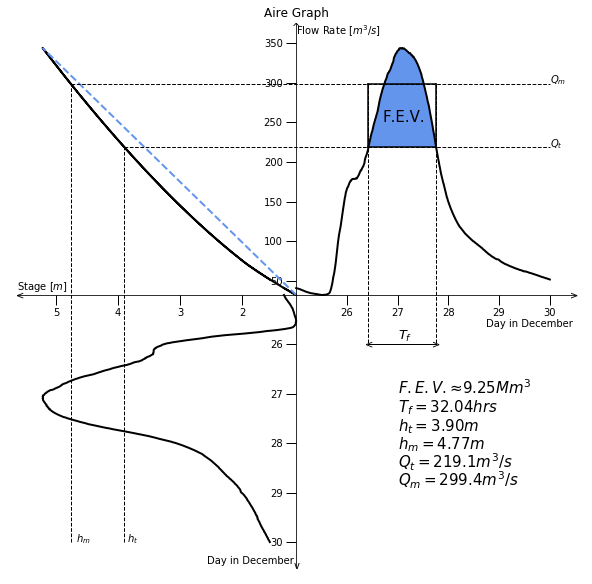
\includegraphics[width=.5\linewidth]{Aire-Quadrant_Graph.png}
\caption{Graph detailing the relationship between the Height and Flow Rate of the River Aire during the 2015 Boxing Day floods using data provided by the Environment Agency from the monitoring station 'Armley'.}
\end{center}
\end{figure}

\subsection{Explanation of the Graph}
In order to plot this graph, we used data showing the stage (stage means height) in metres of the River Aire from the beginning of the 25\textsuperscript{th} until the end of the 30\textsuperscript{th} of December 2015 in 15 minute increments.\\ 

\subsubsection{h\textsubscript{t} and h\textsubscript{m}}
The lower left quadrant shows a plot of stage values against their corresponding time values, which are the only two raw data sets used in this graph. \\
Here, $h_t$ is the threshold stage, i.e. the height at which the river burst its banks and began to flood. $h_t$ can be approximated through a variety of approaches, including using online resources such as gaugemap.co.uk to estimate the height at which a river could begin to flood and social media to find pictures of the river beginning to flood and using the time at which these photos were posted to find the corresponding stage value for the estimated time at which the river began flooding. In this case, Professor Onno Bokhove witnessed the River Aire begin to flood around 10:00 on the 26\textsuperscript{th} of Decmber 2015 at Armley in Leeds.\\
$h_m$ is the mean stage of the river after it has begun to flood. We calculated this by taking all the stage values that are numerically larger than $h_t$, adding up all these values and dividing that sum by the number of said values: \[\frac{\Sigma_{i=1}^{n} h_i}{n},\forall h_i\geq h_t\]\\

\subsubsection{Rating Curve}
For each different gauging station, the environment agency can provide rating information which can be used to define a function Q with which the flow rate of the river can be calculated from a given stage. The general function is defined as:
\[{\bf Q}(h)=c(h-a)^b\]
where c, a and b are provided by the Environment Agency and vary for each gauging station and for different stage intervals. For example, the rating information for the River Aire's Armley station is:
\begin{center}
\begin{tabular}{|l|l|l|l|l|}
\hline
Lower Stage Limit {[}m{]} & Upper Stage Limit {[}m{]} & c & b & a \\
\hline
0.2 & 0.685 & 30.69 & 1.115 & 0.156 \\
0.685 & 1.917 & 27.884 & 1.462 & 0.028 \\
1.917 & 4.17 & 30.127 & 1.502 & 0.153 \\
\hline
\end{tabular}
\end{center}
By running each of our stage values through {\bf Q}(h) as defined for the desired time segment, we compiled a set of time values, their corresponding stage values and their corresponding flow rate values also. This allowed us to plot the rating curve (in the upper right quadrant) and also to plot the flow rate against the time values (in the upper left quadrant). \\
As the provided final upper stage of the rating curve is said to be 4.17 but our maximum stage value is clearly above this, we have had to extrapolate this total upper stage limit to include stage values larger than 4.17.

\subsubsection{Q\textsubscript{t} and Q\textsubscript{m}}
We have now defined the meaning of {\bf Q}(h) and so it is very simple to derive Q\textsubscript{t} as being {\bf Q}(h\textsubscript{t}) and, simlarly, Q\textsubscript{m} as being {\bf Q}(h\textsubscript{m}). As h\textsubscript{t} is 3.90, we use the c, b and a values as defined in the last row of our rating information table.

\subsubsection{T\textsubscript{f} and F.E.V.}
As we have deduced the time, stage and flow rate at which the river begins to flood, it is logical to think that the time from which the flow rate increases above Q\textsubscript{t} to when the flow rate decreases back below Q\textsubscript{t} is the length of time for which the river is actively flooding. This is said to be T\textsubscript{f}.\\ 
It is therefore sensible to assume that the excess flow rate (i.e. the collective flow rate values above our threshold flow rate (Q\textsubscript{t})) multiplied by the length of the flood (T\textsubscript{f}) gives the Flood Excess Volume (F.E.V.). This is the excess volume of water above that maximal capacity of the river that is actually causing the flood and can be seen on our graph as the shaded area between {\bf Q}(h) and Q\textsubscript{t} for the duration of the flood.\\
A good approximation of the F.E.V. can be found using our mean excess flow rate (Q\textsubscript{m}) and multiplying this by T\textsubscript{f}:
\[{\bf F.E.V.}\approx\ T_f (Q_m - Q_t)\]
This constitutes the area of the bold box connecting Q\textsubscript{m}, Q\textsubscript{t} and T\textsubscript{f} on our graph.

\subsection{River Aire}
Having thoroughly explained the various elements of our graph and how they are derived, we can now begin to analyse the data. As can be seen from Figure 1, our estimated F.E.V. is $\approx$ 9.25Mm\textsuperscript{3} and so this is the total volume of fluid that activley caused the flooding at the Armley gauging station in Leeds during the Boxing Day 2015 floods. In section 3 we will investigate how effective flood alleviation schmes, as proposed by the Leeds City Council, at will, in theory, be at stopping this same excess of fluid from causing flooding in the future.

\subsection{The River Calder}
\begin{figure}[H]
\begin{center}
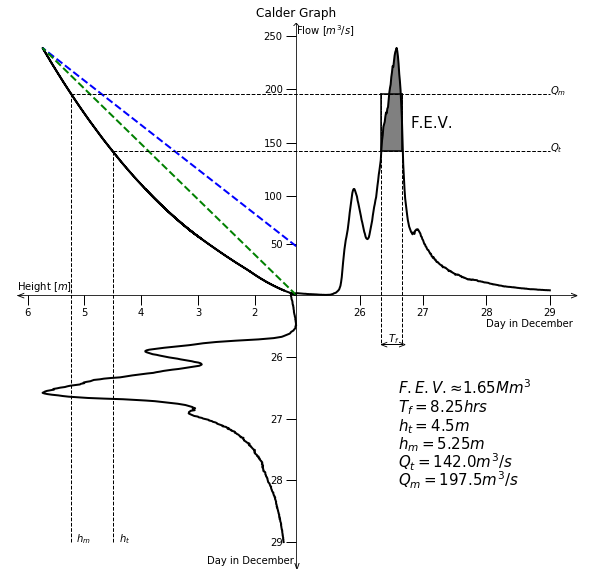
\includegraphics[width=.5\linewidth]{Calder-Quadrant_Graph.png}
\caption{Graph detailing the relationship between the Height and Flow Rate of the River Calder during the 2015 Boxing Day floods using data provided by the Environment Agency from the monitoring station 'Mytholmroyd'.}
\end{center}
\end{figure}
\subsubsection{T\textsubscript{f} and F.E.V.}
When comparing the River Calder flood to the River Aire flood, it is easily seen that the River Calder flooded for a much smaller length of time (the River Aires' T\textsubscript{f} is 3.88 times longer than the River Calders') and hence the River Calders' F.E.V. is minimal in comparison to the River Aire's.
\subsubsection{Rating Curve}
This is the rating information, provided by the Environment Agency for the time of the Boxing Day floods, that we used to calculate the flow rate of the River Calder:
\begin{center}
\begin{tabular}{|l|l|l|l|l|}
\hline
Lower Stage Limit {[}m{]} & Upper Stage Limit {[}m{]} & c & b & a \\
\hline
0 & 2.107 & 8.459 & 2.239 & 0.342 \\
2.107 & 3.088 & 21.5 & 1.37 & 0.826 \\
3.088 & 5.8 & 2.086 & 2.515 & -0.856 \\
\hline
\end{tabular}
\end{center}

\subsection{The River Don}
\begin{figure}[H]
\begin{center}
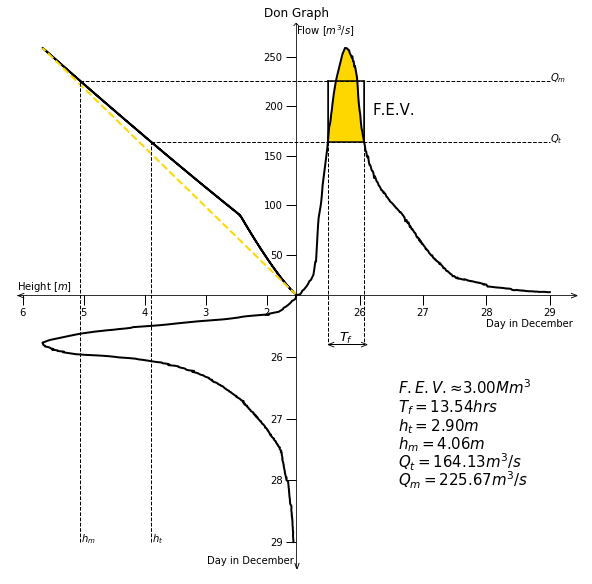
\includegraphics[width=.5\linewidth]{Don-Quadrant_Graph.png}
\caption{Graph detailing the relationship between the Height and Flow Rate of the River Don during the 2015 Boxing Day floods using data provided by the Environment Agency from the monitoring station 'Sheffield Hadfields'.}
\end{center}
\end{figure}
\subsubsection{T\textsubscript{f} and F.E.V.}
The duration of the flood of the River Don is, much like the River Calder, significantly shorter than the River Aires' duration. This has also meant that the River Don has a much smaller F.E.V. than the River Aire but the fact that the River Dons' T\textsubscript{f} is slightly larger than the River Calders' means that it does still have a slightly bigger F.E.V. than the River Calder. \\
However, it is clear the the flooding in Leeds from the River Aire was the most substantial, both in regards to the duration of the flooding (T\textsubscript{f}) and the volume of fluid discharged by the flood (F.E.V.).\\
\subsubsection{Rating Curve}
This is the rating information, provided by the Environment Agency for the time of the Boxing Day Floods, that we used to calculate the flow rate of the River Don:
\begin{center}
\begin{tabular}{|l|l|l|l|l|}
\hline
Lower Stage Limit {[}m{]} & Upper Stage Limit {[}m{]} & c & b & a \\
\hline
0 & 0.52 & 78.4407 & 1.7742 & 0.223 \\
0.52 & 0.931 & 77.2829 & 1.3803 & 0.3077 \\
0.931 & 1.436 & 79.5956 & 1.2967 & 0.34 \\
1.436 & 3.58 & 41.3367 & 1.1066 & -0.5767 \\
\hline
\end{tabular}
\end{center}

\newpage
\section{Flood Mitigation Schemes in Leeds}

\newpage
\section{Analysis of the 2012 November floods}
Flooding is an issue that continues to plague the county of Warwickshire, in particualr Warwickshire is at high risk from river flooding and surface water flooding. In fact, "around one in seven commercial properties and one in ten residential properties are at risk from flooding from rivers or surface water" \cite{5} meaning that, statistically, "the fear of flooding is greater than the fear of crime in large areas of the county" \cite{5}. Numerous flooding events in recent history confirm the risk that Warwickshire faces from flooding, these include:
\begin{itemize}
\item January 1992
\item Easter 1998
\item August 1999
\item June 2005
\item June/July 2007
\item December 2008
\item November 2012
\item July 2014
\end{itemize}
In our analysis, we will be focussing specifically on the November 2012 floods.

\subsection{The River Avon at Stratford-upon-Avon}
\begin{figure}[H]
\begin{center}
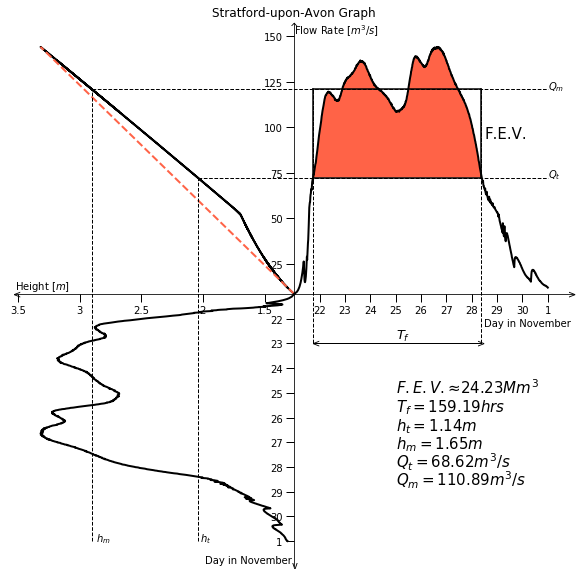
\includegraphics[width=.5\linewidth]{Stratford-Quadrant_Graph.png}
\caption{Graph detailing the relationship between the Height and Flow Rate of the River Avon during the 2012 November floods using data provided by the Environment Agency from the monitoring station at 'Cox's Yard'.}
\end{center}
\end{figure}
\subsubsection{h\textsubscript{t}}
We have devised a very rough manner of approximating h\textsubscript{t} and this is by using gaugemap.co.uk \cite{6}. This is a goverment run website and it provides river information for a specified locale, which in this case is the River Avon at Stratford-upon-Avon. The website also states that flooding may occur from $\approx$ 0.95m.By adding on a 20\% uncertainty, we estimate our threshold stage (h\textsubscript{t}) to be $\approx$ 1.14m.
\subsubsection{T\textsubscript{f} and F.E.V.}
Through our analysis, it can be seen that the length of the flood (T\textsubscript{f}) is 159.19 hours which is equivalent to a 6 day and 15 hour flood, significantly longer than the Boxing Day 2015 floods we investigated in section 2 which on average only had floods of length 17.95 hours. As a result, the estimation for the F.E.V. of the November 2012 floods in Stratford-upon-Avon is vastly larger than for our Boxing Day floods (24.23Mm\textsuperscript{3} in comparison to an average of 4.62Mm\textsuperscript{3} between the three Boxing Day floods) despite both the maximum flow rate and stage (131.03m\textsuperscript{3}/s and 1.89m respectively) being much lower than the averages for the Boxing Day floods (210.71m\textsuperscript{3}/s and 5.21m respectively).
\subsubsection{Rating Curve}
The Environment Agency provided us with the rating information for the Stratford-upon-Avon station for the time of the November 2012 floods. This was particularly important for this location as this station is the only one we have analysed that did not record the flow rate as well as the stage, thereby making the rating information essential to predicting the flow rate of the River Avon at Stratford-upon-Avon at the time of the flood.\\
\begin{center}
\begin{tabular}{|l|l|l|l|l|}
\hline
Lower Stage Limit {[}m{]} & Upper Stage Limit {[}m{]} & c & b & a \\
\hline
0.136 & 0.938 & 158.04 & 2.85438 & 0.262919 \\
0.938 & 1.427 & 87.0362 & 0.962129 & 0.358741 \\
\hline
\end{tabular}
\end{center}
We were also advised by the Environment Agency that the rating at Stratford-upon-Avon is not very accurate and so may have a degree of error to the flow rate predictions it provides.

\subsection{The River Avon at Warwick}
\begin{figure}[H]
\begin{center}
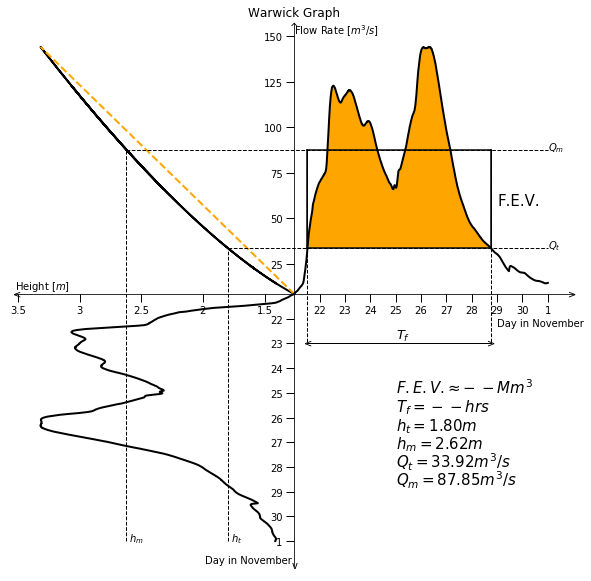
\includegraphics[width=.5\linewidth]{Warwick-Quadrant_Graph.png}
\caption{Graph detailing the relationship between the Height and Flow Rate of the River Avon during the 2012 November floods using data provided by the Environment Agency from the monitoring station at 'Warwick'.}
\end{center}
\end{figure}
\subsubsection{h\textsubscript{t}}
In much the same way we estimated the h\textsubscript{t} of the River Avon in Stratford-upon-Avon, we used gaugemap.co.uk \cite{7}, which gave us an estimate for the height at which flooding may occur to be $\approx$ 1.5m and, by adding on a 20\% uncertainty, we approximated h\textsubscript{t} to be $\approx$ 1.80m.
\subsubsection{T\textsubscript{f} and F.E.V.}
Because we are analysing the same flood along the same river in two different locations, it should be expected for the two floods to have similar characteristics. This can be seen from the fact that the two floods have very similar lengths, with the flood in Warwick only lasting an estimated 8.89\% longer than the flood in Stratford-upon-Avon.\\ However, there is a more significant difference in the F.E.V. between the two floods. In fact, Warwicks' F.E.V. is estimated to be a full 38.88\% larger than Stratford-upon-Avons'. This can be atributed to a number of reasons, the most significant one being the difference between the estimated Q\textsubscript{t} and Q\textsubscript{m} for each flood.\\
This can be deduced from our formula for the Flood Excess Volume:
\[{\bf F.E.V.}\approx\ T_f (Q_m - Q_t)\]
Therefore, because we know that the T\textsubscript{f}s are comparable between the two floods, we can see that the only factor that would constitute a large difference in our approximation for F.E.V. would be a large difference in the value given by Q\textsubscript{m} $-$ Q\textsubscript{t} for each flood. Indeed, the difference for each flood is:
\[
\begin{cases}
\ \ \ \text{\bf Warwick} = Q_m-Q_t = 87.85m^3 /s-33.92m^3 /s = 53.93m^3 /s\\
\ \ \ \text{\bf Stratford-upon-Avon} = Q_m-Q_t = 110.89m^3 /s-68.62m^3 /s = 42.27m^3 /s\\
\end{cases}
\]
\subsubsection{Rating Curve}
The rating information provided by the Environment Agency for Warwick at the time of the November 2012 floods is:
\begin{center}
\begin{tabular}{|l|l|l|l|l|}
\hline
Lower Stage Limit {[}m{]} & Upper Stage Limit {[}m{]} & c & b & a \\
\hline
0.960 & 3.000 & 40.6178 & 1.44854 & 0.917837 \\
\hline
\end{tabular}
\end{center}
This rating information is different from every other set provided for each station analysed in this report as there is only one set of co-efficients. By comparing the Figure 5 with the same graph but using raw flow rate data provided by the Environment Agency as opposed to using the rating information to plot the flow rate:
\begin{figure}[h!]
\centering
\subfloat[Figure 5]{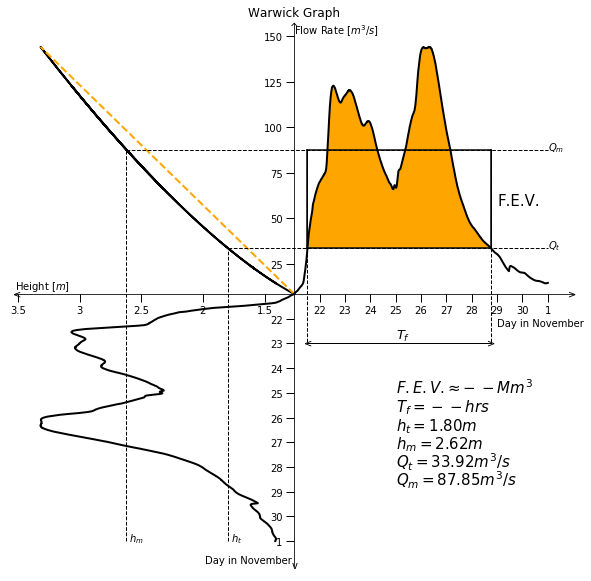
\includegraphics[width=0.5\textwidth]{Warwick-Quadrant_Graph.png}}
\hfill
\subfloat[Figure 5 plotted using raw flow rate data]{\includegraphics[width=0.5\textwidth]{Warwick-Quadrant_Graph_2.png}}
\caption{Comparison of the Warwick graph, the left usng our rating information to find our flow rate values and the right using raw flow rate data.}
\end{figure}\\
we can see that there is negligble difference between the two graphs meaning the rating information has a high degree of accuracy. However, this also raises an interesting question, the question of whether the Environment Agency does indeed collect raw flow rate data or instead uses the rating information to calculate the flow rate.


\newpage
\section{Flood Mitigation Schemes in Warwickshire}
In 2016, Warwickshire County Council published the Warwickshire Local Flood Risk Management Strategy \cite{5}, which had 4 stated objectives, one being to "seek to reduce local flood risk in Warwickshire in an economically, socially and environmentally sustainable way" \cite{5}. \\
As part of this strategy, we know that \pounds1.1 million has been granted by the County Council for the sole purpose of flood alleviation alongside the establishment of the Flood Risk Management team. We also know that Severn Trent Water has delivered \pounds22 million of flood alleviation to Warwick and Leamington Spa. The Countryside Stewardship scheme also allocates a maximum of \pounds6800 per hectare for the planting of new woodland, which, as mentioned in section 1.2, is a type of Natural Flood Management.\\
The next steps of this report will be to investigate which flood mitigation schemes this investement is being used on and by how much each flood mitigation scheme will reduce the F.E.V. produced by the floods in 2012 for both Warwick and Stratford-upon-Avon, in much the same way we analysed the flood mitigation schemes proposed by the Leeds City Council to combat flooding along the River Aire in Section 3.

\newpage
\section{References}
\begin{thebibliography}{}
\bibitem{1}The Flood and Coastal Defence project of the Forsight programme2004: Foresight, Future Flooding. Archived at https://assets.publishing.service.gov.uk/government/uploads/system/uploads/attachment\textunderscore data/file/300332/04-947-flooding-summary.pdf
\bibitem{2}The Telegraph 2015: UK flooding: cost of damage to top £5bn but many homes and businesses underinsured. https://www.telegraph.co.uk/finance/economics/12071604/UK-flooding-cost-of-damage-to-top-5bn-but-many-homes-and-businesses-underinsured.html
\bibitem{3} Peters, H. 1990: Tattooed Faces and Stilt Houses: Who Were the Ancient Yue? Archived at http://sino-platonic.org/complete/spp017\textunderscore yue.pdf
\bibitem{4}Warwickshire County Council 2016: Surface Water Management Plan Methodology Report. Archived at https://apps.warwickshire.gov.uk/api/documents/WCCC-1039-45
\bibitem{5}Warwickshire County Council 2016: Local Flood Risk Management Strategy. Archived at https://apps.warwickshire.gov.uk/api/documents/WCCC-1039-29
\bibitem{6}Stratford. https://www.gaugemap.co.uk/\#!Detail/47
\bibitem{7}Warwick. https://www.gaugemap.co.uk/\#!Detail/45
\end{thebibliography}

\newpage
\appendix
\section{Appendix}
{\bf The Aire Quadrant Graph - Python Code:}\\
{\em Should I include all data sets and code for each graph?}
\begin{lstlisting}
import matplotlib.pyplot as plt
import pandas as pd
import numpy as np

plt.rcParams["figure.figsize"] = [10,10]
plt.rcParams['axes.edgecolor']='white'
fig, ax = plt.subplots()

#Import the Data
armley=pd.read_csv('Aire Data.csv')
day = armley['Day in December']
flow = armley['Flow Rate (m^3/s)']
height = armley['Height (m)']

#Scale our Data
def scale(x):
    return ((x-min(x))/(max(x)-min(x)))
scaledday = scale(day)
scaledheight = scale(height)

#finding and using ht from the hm.
ht=3.9
HM = []
for i in height:
    if i>=ht:
        HM.append(i)
hm=sum(HM)/len(HM)

#Finding qt and qm.
def Q(x):
    if x<=0.685 and x>=0.165:
        y = (30.69*((x-0.156)**1.115))
    elif x<=1.917 and x>0.685:
        y = (27.884*((x-0.028)**1.462))
    elif x<=max(height) and x>1.917:
        y = (30.127*((x-0.153)**1.502))
    return(y)
qt = Q(ht)
qm = Q(hm)   

#Rating Curve
Flow = []
for i in height:
    if i<=0.685 and i>=0.165:
        Flow.append(30.69*((i-0.156)**1.115))
    elif i<=1.917 and i>0.685:
        Flow.append(27.884*((i-0.028)**1.462))
    elif i<=max(height) and i>1.917:
        Flow.append(30.127*((i-0.153)**1.502))

scaledFlow = []
for i in Flow:
    scaledFlow.append((i-min(Flow))/(max(Flow)-min(Flow)))


#Plot the Rating Curve using Q NOT the Flow Rate.
negheight = -scaledheight
ax.plot(negheight,scaledFlow,'black',linewidth=2)
ax.plot([0,-1],[0,1],'cornflowerblue',linestyle='--', marker='', linewidth=2)
#Originally the dotted line was wrong because it went to the positional origin
#and not the actual origin.

#Plot the Flow Rate and Height against the Date.
negday = -(scaledday)
ax.plot(scaledday, scaledFlow, 'black', linewidth=2)
ax.plot(negheight, negday, 'black', linewidth=2)

#Plot the lines illustrating ht,hm,qt,qm
#Scaling ht,hm,qt and qm.
scaledht = (ht-min(height))/(max(height)-min(height))
scaledhm = (hm-min(height))/(max(height)-min(height))
scaledqt = (qt-min(Flow))/(max(Flow)-min(Flow))
scaledqm = (qm-min(Flow))/(max(Flow)-min(Flow))
ax.plot([-scaledht,-scaledht],[-1,scaledqt], 'black', linestyle='--', linewidth=1)
ax.plot([-scaledhm,-scaledhm],[-1,scaledqm], 'black', linestyle='--', linewidth=1)
ax.plot([-scaledht,1],[scaledqt,scaledqt], 'black', linestyle='--', linewidth=1)
ax.plot([-scaledhm,1],[scaledqm,scaledqm], 'black', linestyle='--', linewidth=1)

#Fiddly plot to plot the box around the F.E.V. and the Tf line.
ax.plot([71/250,71/250,71/250],[scaledqt,scaledqm,-1/5], 'black', linestyle='--', linewidth=1)
ax.plot([69/125,69/125,69/125],[scaledqt,scaledqm,-1/5], 'black', linestyle='--', linewidth=1)
ax.plot([71/250,69/125],[-1/5,-1/5], 'black', linewidth=1)
ax.plot([71/250,71/250],[scaledqm,scaledqt], 'black',linewidth=1.5)
ax.plot([71/250,69/125],[scaledqm,scaledqm], 'black',linewidth=1.5)
ax.plot([71/250,69/125],[scaledqt,scaledqt], 'black',linewidth=1.5)
ax.plot([69/125,69/125],[scaledqm,scaledqt], 'black',linewidth=1.5)

#Formatting the ticks and the Axis.
ticks_x = [-3874/4091,-2874/4091,-1874/4091,-874/4091,1/5,2/5,3/5,4/5,1]
#This describes the position I want each tick to be on a graph with x axis
#from -1 to 1. Done by doing (2-min(height))/(max(height)-min(height))
#to find where 2 should be positioned on the axis.
ticks_y = [-1,-4/5,-3/5,-2/5,-1/5,3/52,17/78,59/156,7/13,109/156,67/78,53/52]
ax.set_xticks(ticks_x)
ax.set_yticks(ticks_y)
Ticks_x = [5,4,3,2,26,27,28,29,30]
Ticks_y = [30,29,28,27,26,50,100,150,200,250,300,350]
ax.set_xticklabels(Ticks_x)
ax.set_yticklabels(Ticks_y)
ax.spines['left'].set_position(('center'))
ax.spines['bottom'].set_position(('center'))
ax.spines['left'].set_color('black')
ax.spines['bottom'].set_color('black')
ax.tick_params(axis='x', colors='black', direction='out', length=10, width=1)
ax.tick_params(axis='y', colors='black', direction='out', length=10, width=1)

#Graph Title.
plt.title('Aire Graph')

#Graph labels.
plt.text(-4/6, -1,'$h_t$')
plt.text(-13/15, -1,'$h_m$')
plt.text(1, scaledqm,'$Q_m$')
plt.text(1, scaledqt,'$Q_t$')
plt.text(0.34,0.70,'F.E.V.', size=15)
plt.text(0.4,-0.18,'$T_f$',size=13)
plt.text(0.27,-0.213,'<')
plt.text(0.535,-0.213,'>')

#Axis Labels.
plt.text(0, 1.05,'Flow Rate $[m^3/s]$', size=10)
plt.text(0.75, -0.13,'Day in December', size=10)
plt.text(-0.35, -1.09,'Day in December', size=10)
plt.text(-1.1, 0.02,'Stage $[m]$', size=10)

#Arrows at end of Axis.
plt.text(-0.015,1.07,'^')
plt.text(-0.011,-1.11,'v')
plt.text(1.08,-0.013,'>')
plt.text(-1.105,-0.013,'<')

#Text on Graph.
plt.text(0.4,-0.4,'$F.E.V.≈9.25Mm^3$', size=15)
plt.text(0.4,-0.475,'$T_f=32.04hrs$', size=15)
plt.text(0.4,-0.55,'$h_t=3.90m$', size=15)
plt.text(0.4,-0.625,'$h_m=4.77m$', size=15)
plt.text(0.4,-0.7,'$Q_t=219.1m^3/s$', size=15)
plt.text(0.4,-0.775,'$Q_m=299.4m^3/s$', size=15)

#Fill in the F.E.V.
QT=[]
for i in scaledFlow:
    i = scaledqt
    QT.append(i)
#Because I have to make qt into a list otherwise I get an error because I'm
#comparing a list with a float.
a=np.array(scaledFlow)
b=np.array(QT)
#Puts lists into an array as opposed to a list. Means that Python finds it easier to
#compare the 2.
ax.fill_between(scaledday,a,b,where=a>=b,facecolor='cornflowerblue')

#Find the Tf
idx = np.argwhere(np.diff(np.sign(b - a))).flatten()
print(scaledday[idx])
def unscaleday(x):
    return (((max(day)-min(day))*x)+min(day))
c=unscaleday(0.283)
d=unscaleday(0.55)
Tf=(d-c)*24
print(Tf)
#find Tf in seconds
Tfs=Tf*(60**2)

#Find F.E.V
FEV=(qm-qt)*Tfs
print(FEV)
\end{lstlisting}

\end{document}